\chapter{Training files}
\label{TrainingFiles}
\section{Configuration Files}
The following are the configuration in yaml format used in the ML-Agents toolkit.

The individual files differ only in the values of the rewards and the size of the test environment (in hunting and escaping, other models use one from common configuration), the other parameters are the same for each test environment and are shown once in common section below.
\\
\\
The meaning of each parameter is described in the documentation for the ML-Agents toolkit \cite{MLAgentsParameterDescription}.

\subsection{Common Configuration}
\begin{lstlisting}
behaviors:
  AgentMovement:
    trainer_type: ppo
    hyperparameters:
      batch_size: 1024
      buffer_size: 10240
      learning_rate: 0.0003
      beta: 0.005
      epsilon: 0.2
      lambd: 0.95
      num_epoch: 3
      learning_rate_schedule: linear
    network_settings:
      normalize: false
      hidden_units: 256
      num_layers: 1
      vis_encode_type: simple
    reward_signals:
      extrinsic:
        gamma: 0.99
        strength: 1.0
    keep_checkpoints: 5
    max_steps: 1000000
    time_horizon: 64
    summary_freq: 10000
environment_parameters:
  is_training: 1

  # features
  agent_speed:
    sampler_type: uniform
    sampler_parameters:
      min_value: 0
      max_value: 100
  agent_sensory_range:
    sampler_type: uniform
    sampler_parameters:
      min_value: 0
      max_value: 100
      
  # training area size
  training_area_size:
    curriculum:
      - name: SmallAreaSize
        completion_criteria:
          measure: progress
          behavior: AgentMovement
          min_lesson_length: 5
          threshold: 0.1
        value: 0.5
      - name: MediumAreaSize
        completion_criteria:
          measure: progress
          behavior: AgentMovement
          min_lesson_length: 5
          threshold: 0.4
        value: 1.0
      - name: LargeAreaSize
        completion_criteria:
          measure: progress
          behavior: AgentMovement
          min_lesson_length: 5
          threshold: 0.7
        value: 2.0
      - name: ExtraLargeAreaSize
        value: 3.0
\end{lstlisting}

\subsection{Drinking Configuration}
\begin{lstlisting}
environment_parameters:
  rabbit_each_episode_fixed: -1.0
  fox_each_episode_fixed: -1.0
  agent_bump_into_wall: -0.2
  agent_bump_into_food: -0.2
  agent_drink_reward: 1.0
\end{lstlisting}

\subsection{Eating Carrot Configuration}
\begin{lstlisting}
environment_parameters:
  rabbit_eating_carrot_reward: 1
  rabbit_each_episode_fixed: -1
  agent_bump_into_wall: -0.2
    agent_bump_into_water: -0.2
\end{lstlisting}

\subsection{Mating Configuration}
\begin{lstlisting}
environment_parameters:
  rabbit_each_episode_fixed: -1
  fox_each_episode_fixed: -1
  agent_bump_into_wall: -0.01
  agent_bump_into_water: -0.01
  agent_bump_into_food: -0.01
  rabbit_mating_reward: 1
  fox_mating_reward: 1
\end{lstlisting}

\subsection{Hunting Configuration}
\begin{lstlisting}
environment_parameters:
  # rewards
  fox_eating_rabbit_reward: 1
  fox_each_episode_fixed: -1
  agent_bump_into_wall: -0.01
  agent_bump_into_water: -0.01
  agent_bump_into_food: -0.01

  # training area size
  training_area_size:
    curriculum:
      - name: SmallAreaSize
        completion_criteria:
          measure: progress
          behavior: FoxMovement
          min_lesson_length: 5
          threshold: 0.15
        value: 1.0
      - name: MediumAreaSize
        completion_criteria:
          measure: progress
          behavior: FoxMovement
          min_lesson_length: 5
          threshold: 0.5
        value: 1.0
      - name: LargeAreaSize
        completion_criteria:
          measure: progress
          behavior: FoxMovement
          min_lesson_length: 5
          threshold: 0.75
        value: 1.0
      - name: ExtraLargeAreaSize
        value: 1.0
\end{lstlisting}

\subsection{Escaping Configuration}
\begin{lstlisting}
environment_parameters:
  # rewards
  rabbit_each_episode_fixed: 1
  rabbit_on_eaten: -1
  agent_bump_into_wall: -0.01
  agent_bump_into_water: -0.01
  agent_bump_into_food: -0.01

  # training area size
  training_area_size: 1.0
\end{lstlisting}

\section{Results}
The graphs were created using the TensorBoard tool. \cite{TensorboardTool}

\begin{figure}[H]
    \centering
    \includegraphics[width=\textwidth]{Images/result_drinking_v2.png}
    \caption{Results of training Drinking model.}
    \label{fig:drinkingTrainingResults}
\end{figure}

\begin{figure}
    \centering
    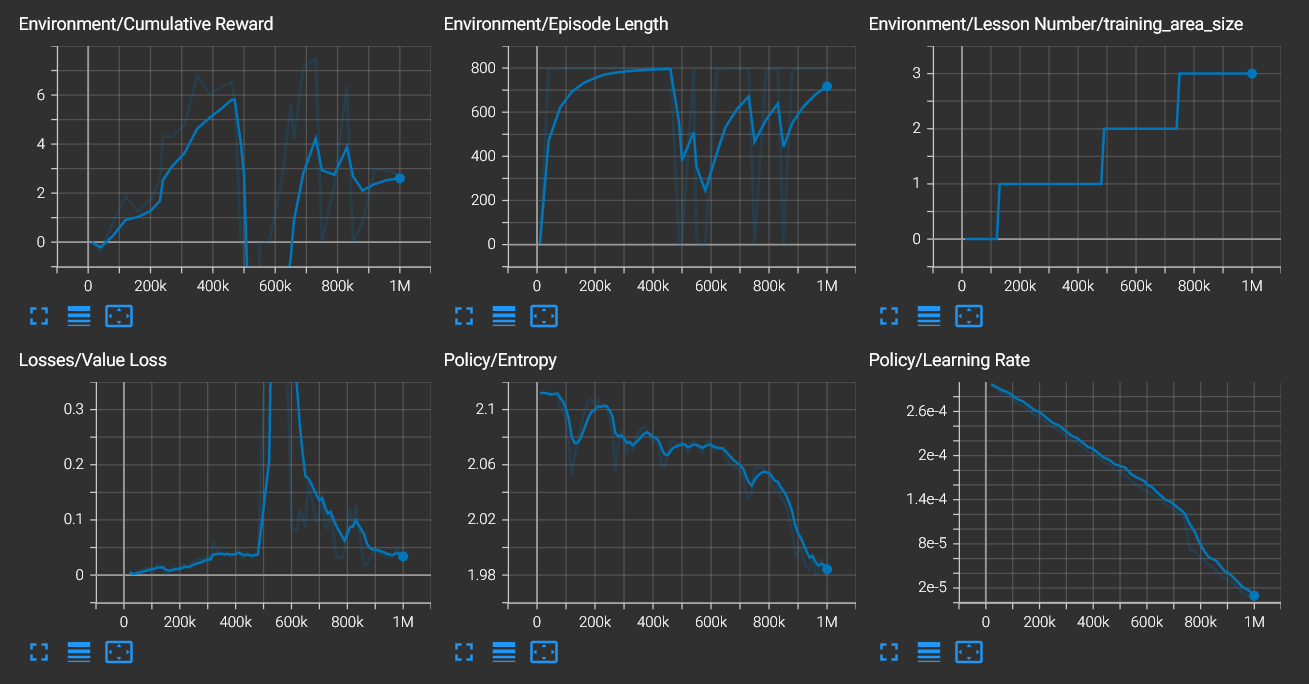
\includegraphics[width=\textwidth]{Images/result_eating_v2.png}
    \caption{Results of training EatingCarrot model.}
    \label{fig:eatingCarrotTrainingResults}
\end{figure}

\begin{figure}
    \centering
    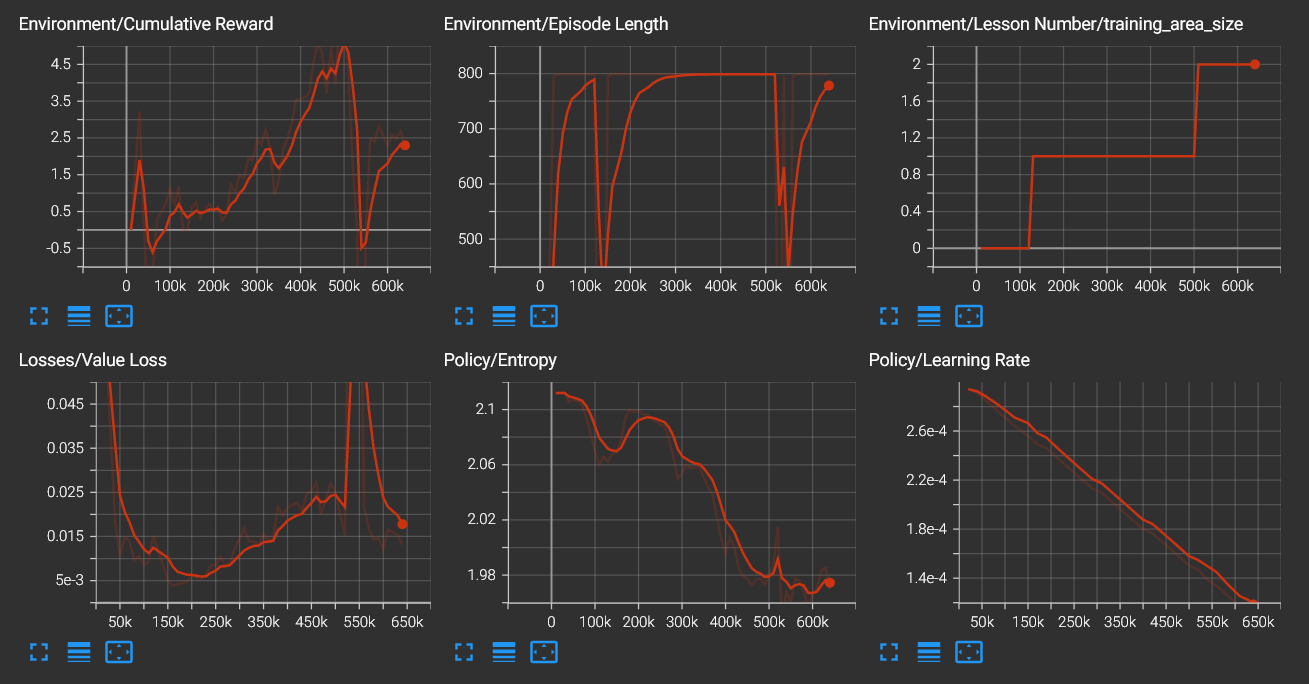
\includegraphics[width=\textwidth]{Images/result_mating_rabbit_v2.png}
    \caption{Results of training Mating-Rabbit model.}
    \label{fig:matingRabbitTrainingResults}
\end{figure}

\begin{figure}
    \centering
    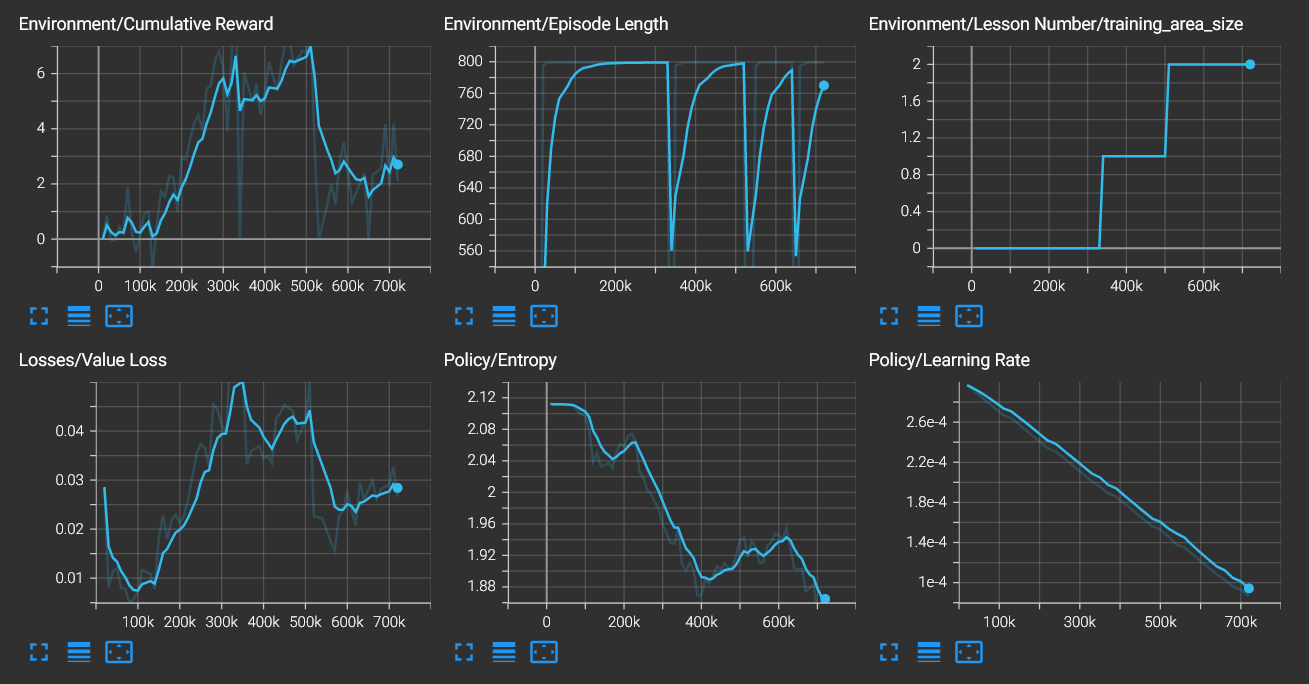
\includegraphics[width=\textwidth]{Images/result_mating_fox_v2.png}
    \caption{Results of training Mating-Fox model.}
    \label{fig:matingFoxTrainingResults}
\end{figure}

\begin{figure}
    \centering
    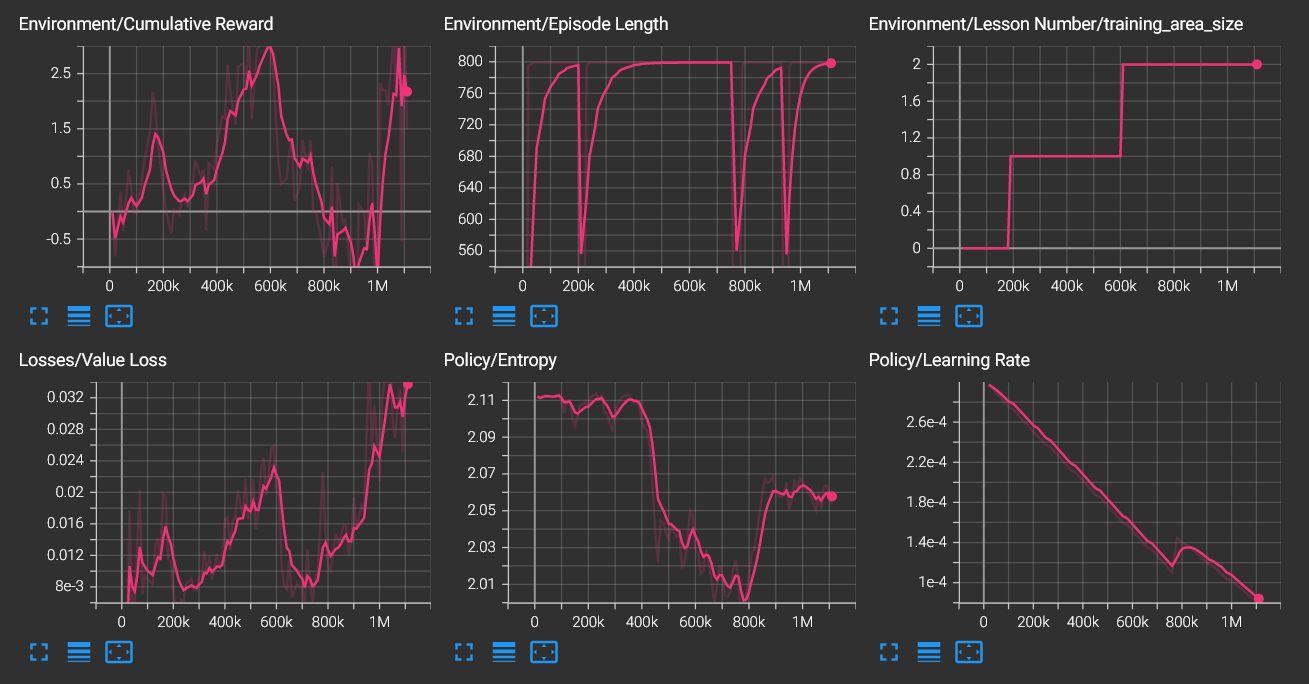
\includegraphics[width=\textwidth]{Images/result_hunting_v2.png}
    \caption{Results of training Hunting model.}
    \label{fig:huntingTrainingResults}
\end{figure}

\begin{figure}
    \centering
    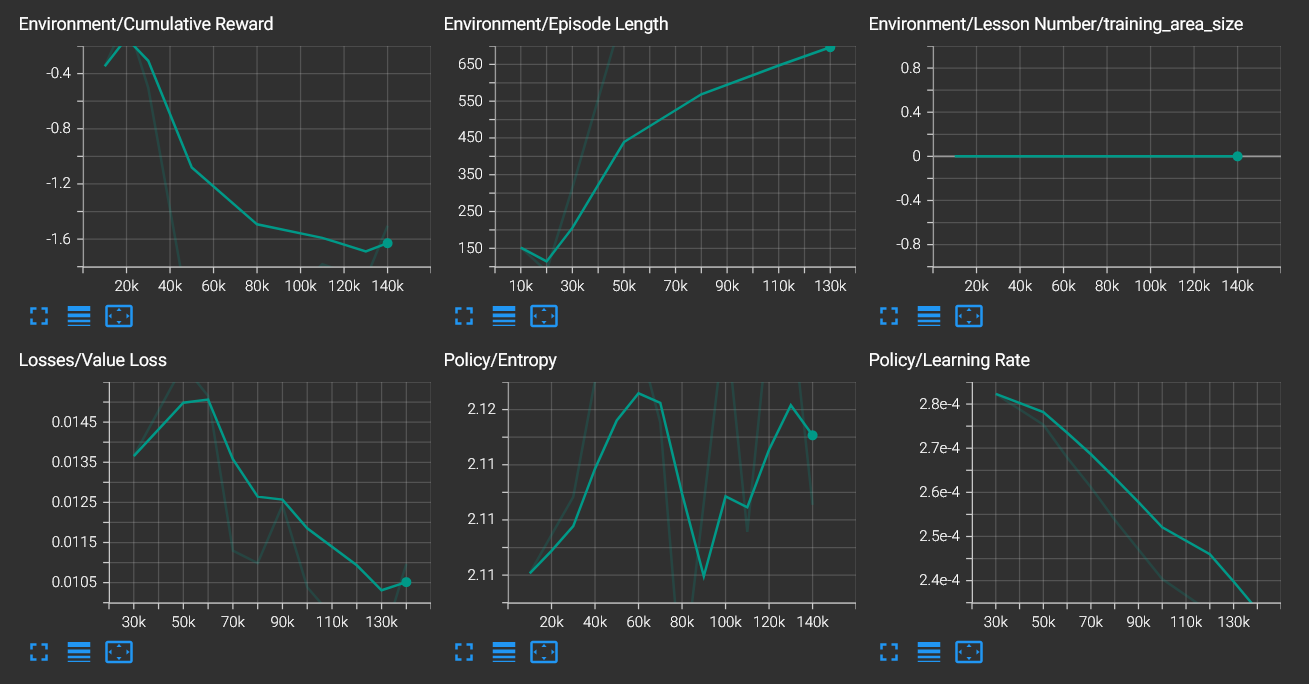
\includegraphics[width=\textwidth]{Images/result_escaping_v2.png}
    \caption{Results of training Escaping model.}
    \label{fig:escapingTrainingResults}
\end{figure}